%%%%%%%%%%%%%%%%%%%%%%%%%%%%%%%%%%%%%%%%%%%%%%%%%%%%%%%%%%%%%%%%%%%
%%% Documento LaTeX 																						%%%
%%%%%%%%%%%%%%%%%%%%%%%%%%%%%%%%%%%%%%%%%%%%%%%%%%%%%%%%%%%%%%%%%%%
% Título:		Capítulo 3
% Autor:  	Ignacio Moreno Doblas
% Fecha:  	2014-02-01, actualizado 2019-11-11
% Versión:	0.5.0
%%%%%%%%%%%%%%%%%%%%%%%%%%%%%%%%%%%%%%%%%%%%%%%%%%%%%%%%%%%%%%%%%%%
% !TEX root = A0.MiTFG.tex

\section{Cuarta iteración: Fiabilidad}
    \subsection{Resumen}
        
        En esta iteración se ha implementado todo lo relacionado con el cálculo de la fiabilidad del algoritmo siguiendo las indicaciones de la norma UNE-EN 60601-2-47:2002. Una vez concluida esta fase del desarrollo el proyecto ya será plenamente funcional, esto es, satisfaciendo todos los requisitos planteados. Aunque se deja para una etapa posterior lo relacionado con las consideraciones de diseño.
        
    \subsection{Requisitos}
    
        Para esta iteración solo se pretende satisfacer un requisito, el 1.3.5 de la tabla inicial (tabla \ref{tab:Requisitos}). Para ello, y tras estudiar el algoritmo propuesto por la norma para determinar la fiabilidad de un detector, se ha dividido el requisito en las diferentes tareas:
        
        \begin{enumerate}
            \item Estudio de la norma \cite{Aenor2002}.
            \item Extraer las anotaciones de la base de datos y añadirlas al fichero de entrada.
            \item Preparar el dispositivo de pruebas para transmitir anotaciones junto a la deteccion de los latidos.
            \item Modificar el algoritmo de detección implementado en la segunda iteración para enviar anotaciones.
            \item Crear un modelo de almacenamiento para las anotaciones que facilite la implementación de la norma. \cite{Aenor2002}
            \item Implementar el control de las anotaciones en el panel de usuario.
            \item Implementar las ecuaciones de cálculo de fiabilidad descritas en la norma. \cite{Aenor2002}
            \item Mostrar al usuario los resultados de la validación del algoritmo.
        \end{enumerate}
    En el siguiente apartado se comenzará con una breve descripción del método propuesto por la norma, antes de abordar la descripción de cada tarea. 
    
    \subsection{Desarrollo}
    
    %Aunque pueda parecer simple, medir la eficiencia de un algoritmo de detección QRS no es sencillo y varía en gran medida en función de los distintos tipos de latidos que se quieran detectar con el algoritmo. En las bases de datos hay numerosos tipos de anotaciones con una amplia variedad de significados, además, es posible que distintas bases de datos empleen diferentes anotaciones para referirse al mismo evento cardíaco.
    
    La norma propone un mecanismo para cuantificar la fiabilidad de un algoritmo de detección de arritmias cardiacas en general, y, básicamente, propone comparar las clasificaciones de los latidos hechas por el algoritmo bajo prueba con las anotaciones contenidas en bases de datos estándar, como la MIT-BIH. 
    
    Así, propone rellenar una tabla como la que aparece en la figura \ref{fig:fiability}, que cruza las anotaciones del algoritmo (minúscula) con las anotaciones de la base de datos (mayúsculas). La nomenclatura que propone la norma para estas anotaciones es: 
    \begin{itemize}
        \item \textbf{N:} Cualquier latido que no sea S,V,F o Q
        \item \textbf{S:} Latido supraventricular o ectópico.
        \item \textbf{V:} Latido ventricular ectópico o prematuro.
        \item \textbf{F:} Mezcla de latido ventricular y normal.
        \item \textbf{Q:} Latido de marcapasos o mezcla de marcapasos y normal.
    \end{itemize}
     
    Un algoritmo con un 100\% de fiabilidad tendría solamente rellena la diagonal de la tabla. El fabricante debe incluir esta tabla en la documentación de su dispositivo.
    
    También, e íntimamente relacionado con la tabla, la norma obliga  a reportar al fabricante dos parámetros relacionados con los falsos positivos y falsos negativos que genera su algoritmo: La predictividad positiva (+P) y la Sensibilidad (Se), respectivamente. Cuando, como es nuestro caso, el algoritmo solo detecta QRS, no hace una posterior calificación, las ecuaciones que la norma propone para determinar ambos parámetros son las de la figura \ref{code:norm}. Como se puede ver, en este caso particular, los QRS detectados correctamente por el algoritmo (QTP) son todos los detectados aunque no hayan sido calificados correctamente. QFN Y QFP, son, respectivamente, el numero de latidos que sí estaban a notados pero el algoritmo no ha detectado (falsos negativos) y los que sí ha detectado, pero no estaban anotados (falsos positivos).
     
    Por último, la norma establece una tolerancia temporal en la comparación del tiempo anotado para el QRS en la base de datos y el tiempo calculado por el algoritmo. 
        
    Por desgracia la nomenclatura de la MIT-BIH no coincide, por lo que, con el objetivo de \textit{extraer las anotaciones de la base de datos}, es necesario hacer algunas conversiones previas. Para ello se han integrado directamente en el script de Matlab implementado durante la primera iteración. Facilitando al usuario final un método de adquirir los datos de la MIT-BIH listos para ser usados. El script resultante puede ser comprobado en el extracto \ref{code:matlabAnn}, y con esto puede darse por finalizada la primera tarea de esta iteración.
        
	\code{Script de Matlab para consultar la base de datos.}{code/GetSampleAsTextWithAnnotations.m}{code:matlabAnn}{Octave}
        
    Para la tercera tarea, \textit{habilitar el envío de anotaciones desde la plataforma de pruebas}, tarea simplemente se ha añadido un nuevo campo al mensaje de tipo ``uint8\char`_t'', que posteriormente será convertido en el panel a ``char''. De momento el algoritmo simple implementado como demostración solo es capaz de notificar latidos con el tipo N, sin embargo el sistema está preparado para que el usuario configure que anotaciones mandar con sus detecciones.
    
    Acompañando a la anterior tarea, se ha \textit{modificado el algoritmo de detección implementado en la segunda iteración}, añadiendo una anotación a cada pico detectado. De esta forma queda preparado para poder ser evaluado mediante la norma. El algoritmo queda representado en el extracto \ref{code:BasicAlgAnn}, como puede observarse apenas hay diferencias con el algoritmo anterior (Extracto \ref{code:BasicAlg}), esto es debido a la simpleza del mismo, ya que solo está detectando latidos normales y por lo tanto todos los latidos detectados son de tipo ``N''.
    
    \code{Algoritmo de detección de picos R sencillo con anotaciones}{code/BasicAlgorithmAnn.c}{code:BasicAlgAnn}{C++}
        
    Para la quinta, \textit{el almacenamiento de las anotaciones}, se ha decidido implementar una clase que contenga todas las funciones necesarias para manejar los datos de las anotaciones. De esta clase se necesita la capacidad de almacenar las anotaciones tanto de la base de datos como de los resultados del algoritmo, la capacidad de calcular las combinaciones de anotaciones en ambas listas y de encontrar aquellas anotaciones que solo están representadas en una de las listas, encontrando con ellas los falsos positivos y negativos. Para facilitar todos estos procedimientos en lugar de listas se han utilizado diccionarios, referidos en QT como QMaps. Empleando el número de la muestra como clave y asignando la anotación al valor. A continuación se describen los diferentes métodos que posee la clase.
        
    A la hora de determinar la fiabilidad es importante determinar la tolerancia de nuestro sistema. Este parámetro será configurable por el usuario desde el panel y vendrá especificado en número de muestras, por lo que dependiendo de la frecuencia de muestreo este corresponderá a un tiempo mayor o menor.

    El mecanismo es sencillo, el número de la muestra se asigna como clave y la anotación como valor. Sin embargo en el caso de las muestras procedentes de los resultados del algoritmo se ha tenido en cuenta el valor de tolerancia para evitar crear varios positivos consecutivos si este oscila en sus resultados. El código puede consultarse en el extracto \ref{code:AddAnn}.
        
    \code{Código para añadir anotaciones.}{code/AddResults.cpp}{code:AddAnn}{C++}

    \textit{El usuario tiene la posibilidad de controlar desde el panel} cuales anotaciones tener en cuenta y cuales no para algoritmos que no busquen satisfacer la norma al completo. Tener alguna de las anotaciones desmarcadas hará que dicha anotación sea tratada como una N, ya que sigue siendo un latido aunque no se desee clasificar el tipo. Además se aprovecha esta función para filtrar de nuevo la existencia de alguna anotación con la nomenclatura errónea para descartarla. El código puede consultarse en el extracto \ref{code:AnnState}.
        
    \code{Código para validar anotaciones.}{code/AnnotationsState.cpp}{code:AnnState}{C++}
        
    Los últimos métodos están relacionados intrínsecamente con el \textit{cálculo de la fiabilidad}, pues según la norma es necesario rellenar una tabla con todas las combinaciones cruzadas de N,S,V,F o Q que se hayan encontrado. Por ello se ha implementado una función con dos tipos de anotaciones como parámetro que calcula todas las ocurrencias de dicha combinación a lo largo de las muestras analizadas. El código puede encontrarse en el extracto \ref{code:CrossSum}. Además se ha implementado una función para calcular los falsos positivos y otra para los falsos negativos, al ser muy similares solo se ha representado una de ellas en el extracto \ref{code:FP}.
        
    \code{Código para calcular la fiabilidad.}{code/CrossSum.cpp}{code:CrossSum}{C++}
    \code{Función para calcular falsos positivos.}{code/FP.cpp}{code:FP}{C++}
  
    \clearpage
    Una vez concluida la gestión interna de los datos resta por implementar la forma de\textit{ mostrar estos al usuario}. Para ello se ha empleado una tabla similar a la indicada por la norma.\cite{Aenor2002} Además se ha incluido un ``checkbox'' a cada fila para activar o desactivar dicha anotación en el calculo de la fidelidad. Como cabe esperar al disponer de 5 tipos de anotaciones la cantidad de combinaciones posibles, al tener en cuenta el orden, es de 25. Como trabajar con 25 salidas de texto diferentes de manera independiente es muy engorroso y difícil de trabajar, estas salidas se han incluido dentro de una matriz y se accede a ellas iterando las celdas de dicha matriz y haciendo un casting al elemento que contiene, observar en el extracto \ref{code:Cast}. 
        
    \code{Código para hacer el casting a elementos de un layout.}{code/casting.cpp}{code:Cast}{C++}
        
    Por ultimo solo queda operar con los valores resultantes de la tabla según la manera indicada por la norma para calcular la fiabilidad en forma de sensibilidad y predictibilidad positiva (Extracto \ref{code:norm}). Una vez calculados, los valores son mostrados al usuario en dos campos de texto. Siendo el resultado final observable en la figura \ref{fig:fiability} y dando por finalizada las tareas a realizar en esta iteración.
        
    \code{Ecuaciones de la norma.}{code/norma.m}{code:norm}{Octave}
        
    \begin{figure}[H]
            \centering
                    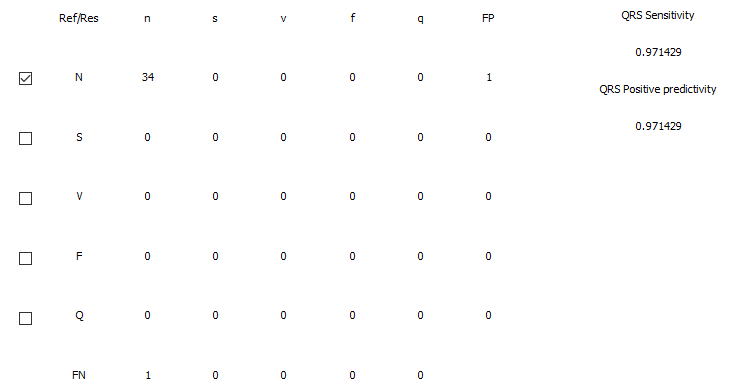
\includegraphics[width = \linewidth]{figuras/fiabilidad.PNG}
            \caption{Calculo de fiabilidad en el panel de usuario.}
            \label{fig:fiability}
    \end{figure}
        
    \subsection{Pruebas}
    
    Las pruebas se han llevado a cabo mediante la implementación de tests unitarios para las diferentes funciones del controlador de las anotaciones. 
    
    En primer lugar se han realizado dos pequeños tests con el objetivo de comprobar dos partes pequeñas pero fundamentales, la escritura y lectura de las anotaciones y la función encargada de realizar las combinaciones. Dichos tests pueden observarse en el extracto \ref{code:AnnUnitTest1}.
    
    \code{Tests unitarios de funciones básicas de las anotaciones}{code/AnnUnitTest1.cpp}{code:AnnUnitTest1}{C++}
    
    Por ultimo se han desarrollado tests que pongan a prueba el funcionamiento completo del sistema de anotaciones. En ellos se proporcionan dos ficheros de entrada conocidos y se confecciona la respuesta adecuada, para después de realizar el proceso comprobar el resultado obtenido con el esperado. Como todos siguen la misma filosofía solo se adjunta uno de ellos en el extracto \ref{code:AnnFromfile}.
    
    \code{Tests unitario de calculo de fiabilidad.}{code/TestAnnotationsFromFile.cpp}{code:AnnFromfile}{C++}
    
    \subsection{Conclusiones}
    
    Durante la realización de esta iteración ha quedado demostrada la necesidad de implementar tests ya que gracias ha ellos se ha podido corregir la implementación de las funciones ``CrossSum'', ``CalculateFP'' y ``CalculateFN'' en hasta tres ocasiones cuando ya se habían dado por finalizadas. De no ser por los tests realizados, muy probablemente los errores hubieran pasado desapercibidos dado lo confusas que pueden llegar a ser estas funciones.